\begin{frame}
  \frametitle{Moltres for MSR Multiphysics Modeling}
  \textbf{What is Moltres?}
  \begin{itemize}
    \item Moltres \cite{lindsay_introduction_2018} is an open-source, MOOSE-based
      multiphysics application for modeling MSRs
	\item \gls{MOOSE} \cite{lindsay_20_2022} is an open source finite-element framework
      that supports the development of multiphysics solvers
    \item Robust and highly scalable numerical routines from PETSc
    \item Flexible coupling capabilities provided by the MOOSE Multi-App system
    \item Highly extensible and user-friendly interface for software development through
      object-oriented programming paradigm in C++ and native compatibility with other MOOSE-based
      apps
  \end{itemize}
\end{frame}

\begin{frame}
  \frametitle{Previous MSR Analyses with Moltres}
  \begin{columns}
    \hfill
    \column[t]{4cm}
      \textbf{\gls{MSRE}}
      \vfill
      \begin{figure}
        \centering
	    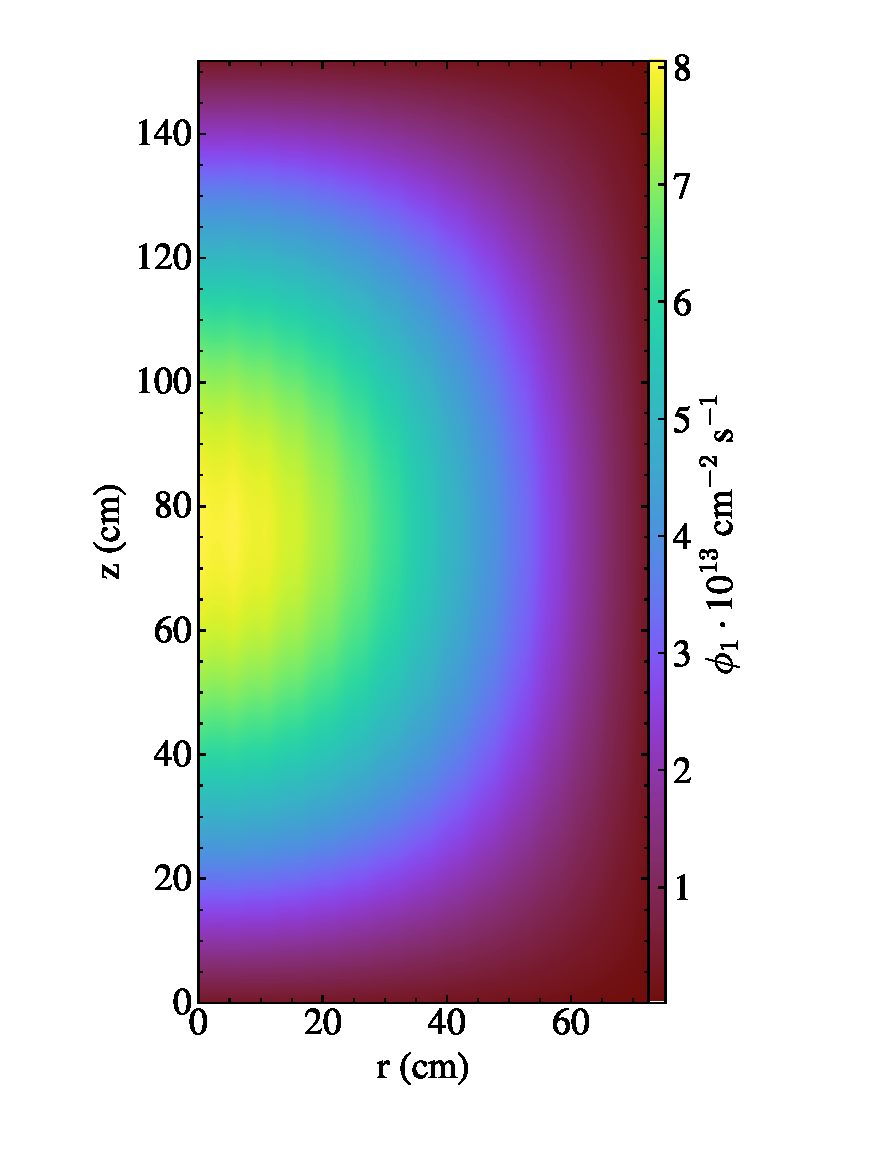
\includegraphics[width=.48\columnwidth]{../images/2d_gamma_heating_group1}
        \hfill
	    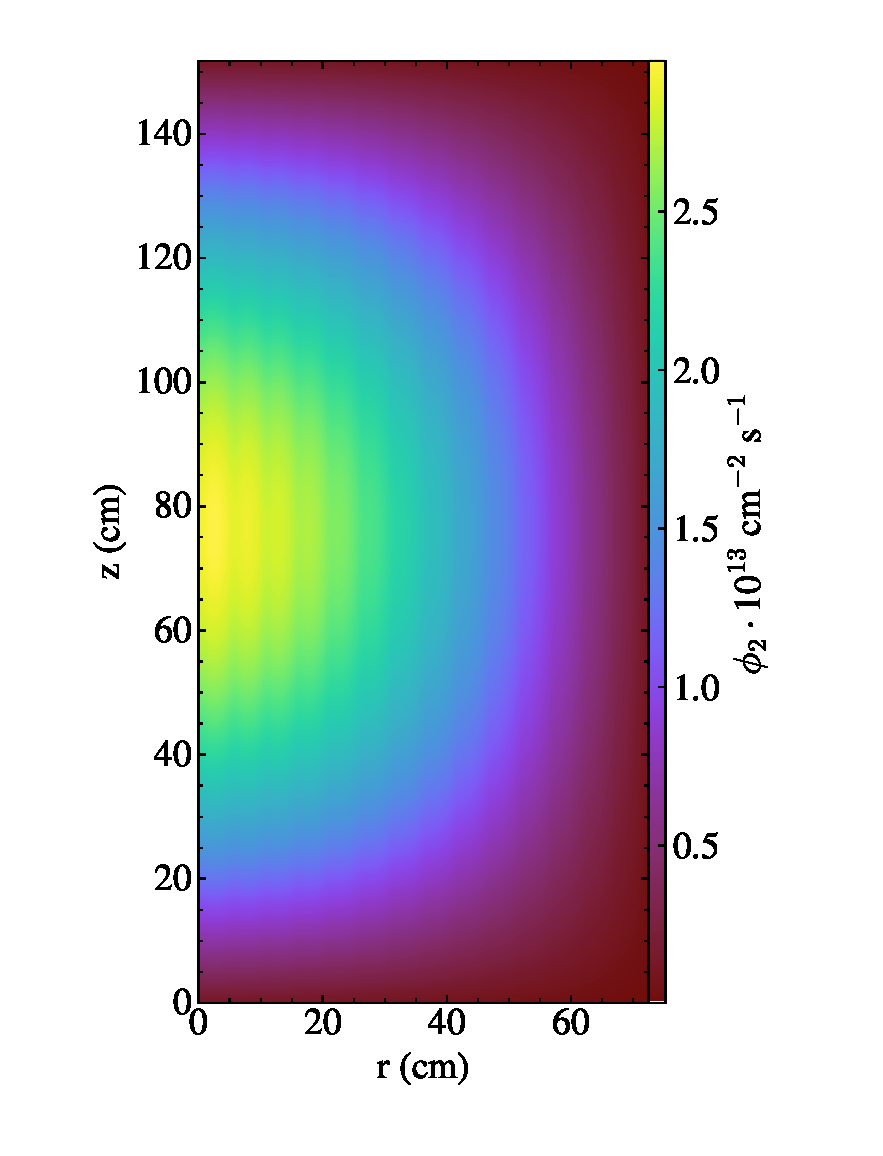
\includegraphics[width=.48\columnwidth]{../images/2d_gamma_heating_group2}
	    \caption{\footnotesize Group 1 and 2 neutron fluxes in a 2-D axisymmetric MSRE
	      model \cite{lindsay_moltres_2017}.}
      \end{figure}
    \hfill
    \column[t]{3.5cm}
      \textbf{\gls{MSFR}}
      \vfill
      \begin{figure}
        \centering
        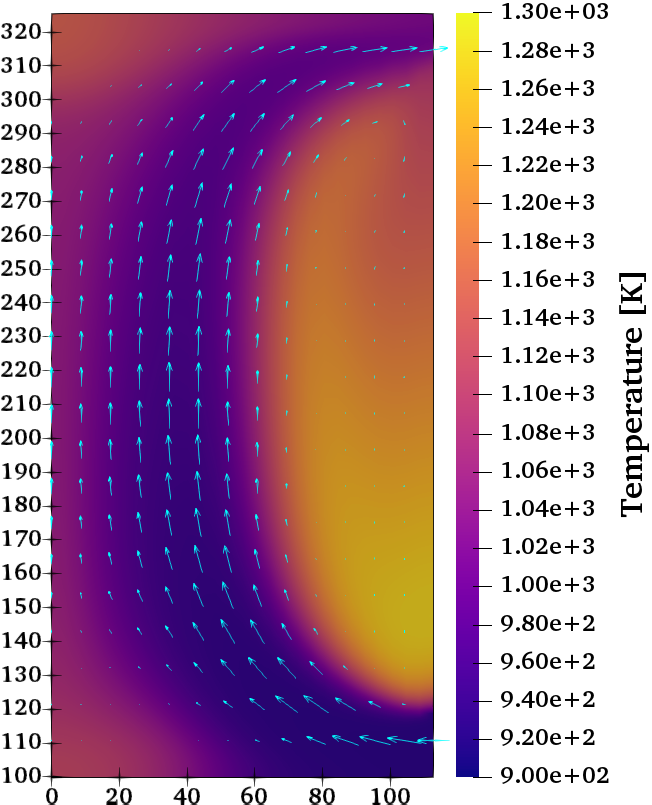
\includegraphics[width=.8\columnwidth]{images/flow-temp-plasma}
        \caption{\footnotesize Steady-state temperature distribution and salt flow velocity fields
          in a 2-D axisymmetric MSFR model. \cite{park_advancement_2020}}
      \end{figure}
    \hfill
    \column[t]{3.5cm}
      \textbf{\gls{TAP} MSR}
      \vfill
      \begin{figure}
        \centering
        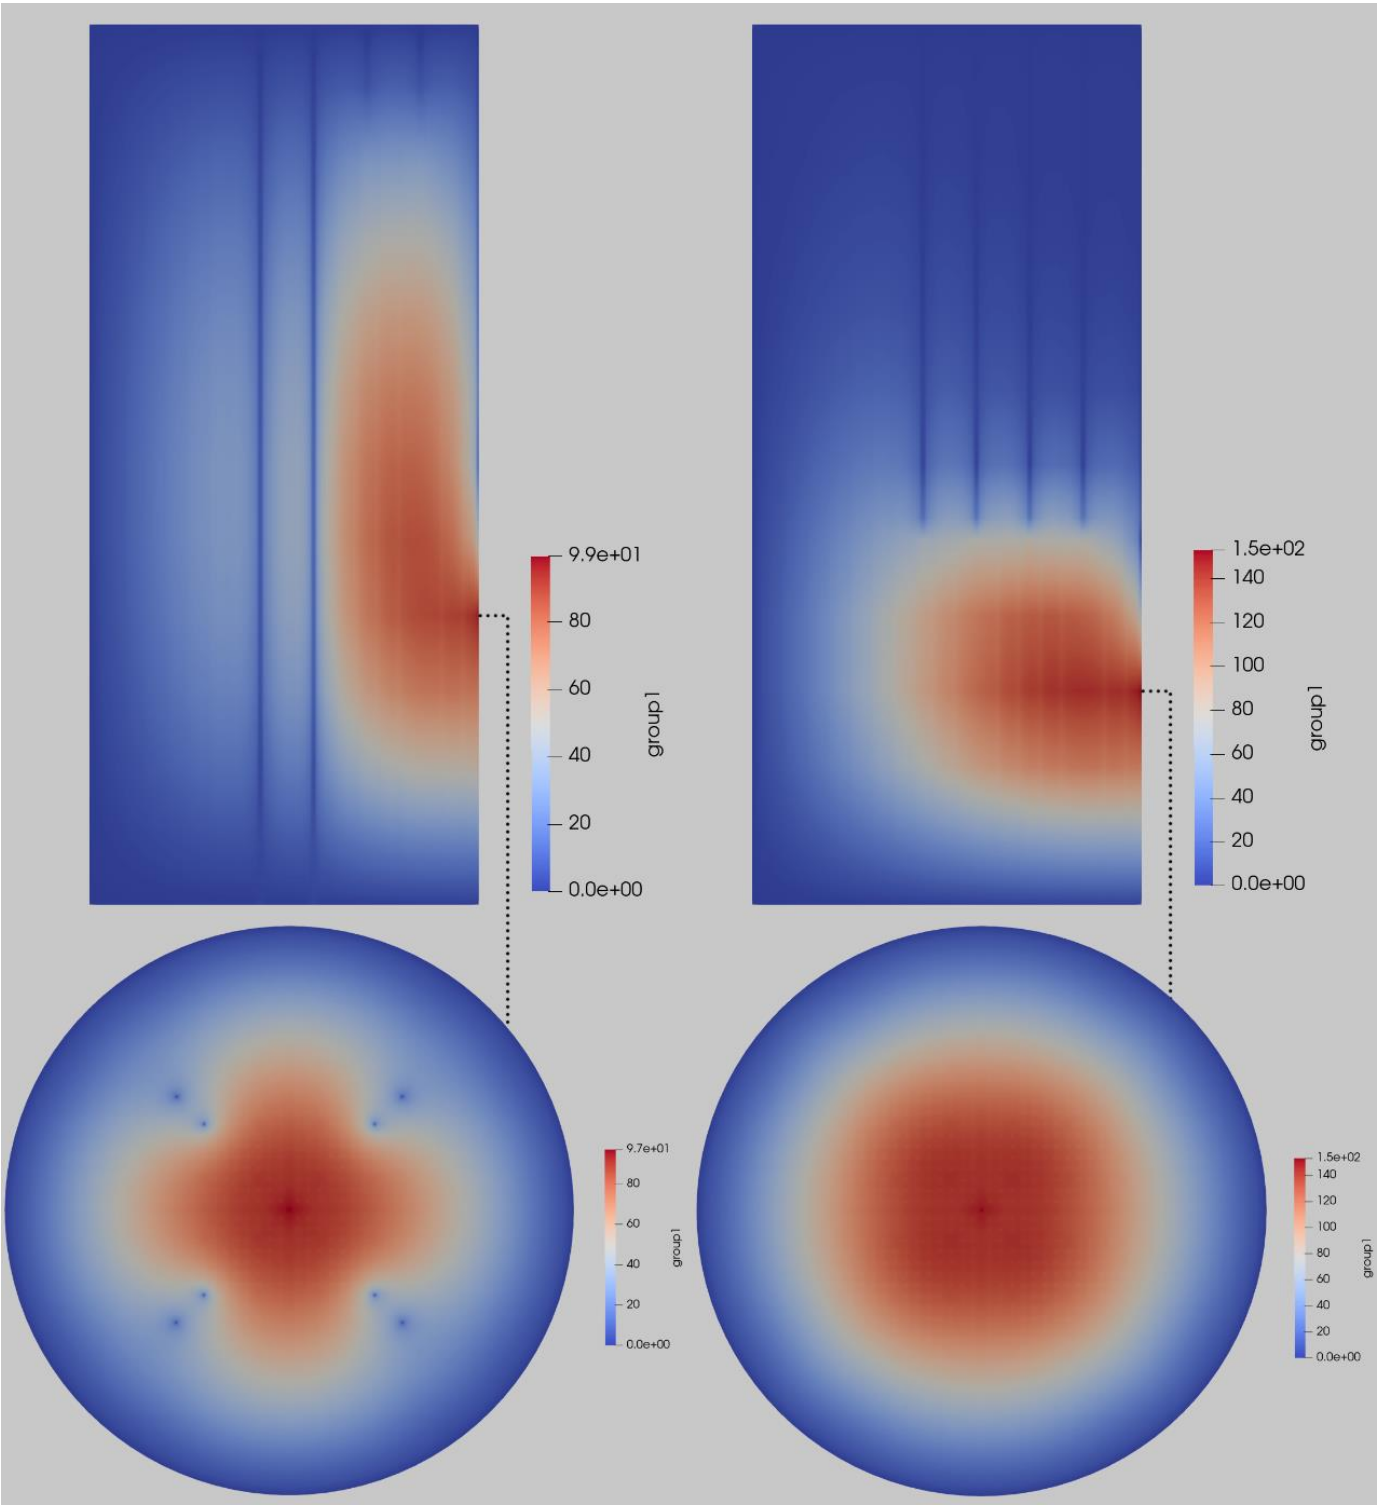
\includegraphics[width=\columnwidth]{images/tap-msr}
        \caption{\footnotesize Group 1 and 2 neutron fluxes in a 3-D TAP MSR model.
        \cite{lee_neutronics_2020}}
      \end{figure}
    \hfill
  \end{columns}
\end{frame}

\begin{frame}
  \frametitle{Moltres}
  \begin{block}{\textbf{Software Capabilities for MSR Modeling}}
    \begin{itemize}
  	  \item Multigroup neutron diffusion solver
      \item Temperature reactivity feedback by interpolating temperature-dependent group
        constant data\footnote{Group constants refer to neutron cross section data and other
        neutronics-related material properties}
      \item \gls{DNP} drift coupling with flow modeling
      \item Out-of-core \gls{DNP} decay
      \item Couples with MOOSE modules for thermal-hydraulics modeling
    \end{itemize}
  \end{block}
  \pause
  \begin{block}{\textbf{Areas of Improvement for Moltres for MSR Modeling}}
    \begin{itemize}
      \item Moltres does not currently have turbulence modeling capability for simulating turbulent
        flows
      \item Moltres cannot model highly neutron-absorbing control rods accurately
    \end{itemize}
  \end{block}
\end{frame}

%\begin{frame}
%  \frametitle{Moltres}
%  \begin{block}<1->{\textbf{Gaps in Moltres Software Development}}
%    \begin{itemize}
%      \item Rigorous verification and validation (V\&V) of existing multiphysics capabilities for
%        MSR modeling
%      \item Turbulence modeling capability for simulating high-Reynolds number flows in MSRs
%    \end{itemize}
%  \end{block}
%  \begin{block}<2->{\textbf{Proposed Work}}
%    \begin{itemize}
%      \item \textbf{Verify and Validate Existing Multiphysics Coupling Capabilities in Moltres}
%      \item \textbf{Implement a RANS-based Turbulence Model in Moltres}
%    \end{itemize}
%  \end{block}
%\end{frame}
